% !TeX spellcheck = fr_FR

% TODO: Replace scan images with clean text where possible

\documentclass[a4paper, 10pt]{report}

\usepackage[french]{babel}
\usepackage[T1]{fontenc}

\usepackage{amsmath, amssymb, amsfonts}

\usepackage{hyperref}
\usepackage{geometry}

\usepackage{xcolor}
\usepackage{graphicx}

\usepackage{fancyhdr}
\usepackage{lastpage}

\usepackage{enumitem}

\geometry{
	a4paper,
	left=25mm,
	right=25mm,
	top=35mm,
	bottom=25mm,
	headsep=5mm,
	headheight=20mm,
}

\definecolor{solution}{HTML}{E5E4E2}
\providecommand{\abs}[1]{\lvert#1\rvert}
\providecommand{\norm}[1]{\lVert#1\rVert}
\DeclareMathOperator{\card}{card}

\makeatletter
\renewcommand*\env@matrix[1][*\c@MaxMatrixCols c]{%
	\hskip -\arraycolsep
	\let\@ifnextchar\new@ifnextchar
	\array{#1}}
\makeatother

\begin{document}
	
	\renewcommand{\headrule}{%
		\vspace{-4pt}\hrulefill
		\raisebox{-6.8pt}{\ 
\includegraphics[height=5mm]{../../icon.png}}
		\hrulefill
	}	
	\pagestyle{fancy}
	\fancyhf{}
	
	\fancyhead[L]{\small \slshape Automne 2024}
	\fancyhead[C]{\Large \bfseries Algèbre I - Série 05}
	\fancyhead[R]{\small Buff Mathias}
	\fancyfoot[L]{
		\small Source files available at:
		\href{https://github.com/MathiasBuff/bsc-math}
		{github.com/MathiasBuff/bsc-math}
	}
	\fancyfoot[R]{
		\small Page \thepage
		\hspace{1pt} /
		\pageref*{LastPage}
	}
	

	\noindent
	\textbf{Exercice 1.}\\
	Résoudre les systèmes linéaires suivants, en travaillant avec les
	matrices correspondantes et leur forme échelonnée :
	
	\[\text{(i)}\left\{\begin{matrix}[rrrcr]
		x & -2y & +3z &=& 1\\
		2x & -3y & +5z &=& 0\\
		-x & +4y & -z &=& 1\\
	\end{matrix}\right.\]
	
	\[\text{(ii)}\left\{\begin{matrix}[rrrcr]
		3x & +y & +z &=& 8\\
		-2x & +y & -3z &=& -22\\
		x & & +z &=& 7\\
		3x & +2y & +z &=& 5\\
	\end{matrix}\right.\]
	
	\[\text{(iii)}\left\{\begin{matrix}[rrrrrrcr]
		x_1 & -5x_2 & -x_3 & +12x_4 & -x_5 & &=& -4\\
		-2x_1 & +10x_2 & +3x_3 & -33x_4 & +2x_5 & +x_6 &=& 4\\
		& & x_3 & -9x_4 & +x_5 & &=& 8\\
		x_1 & -5x_2 & +2x_3 & -15x_4 & +2x_5 & +x_6 &=& 14\\
	\end{matrix}\right.\]
	
	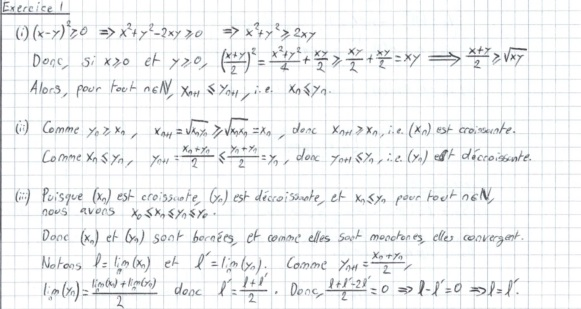
\includegraphics{ex01.jpg}
		
	\newpage
	
	\fancyhf{}
	\renewcommand{\headrule}
	{\rule{\textwidth}{0pt}}
	\fancyfoot[R]{
		\small Page \thepage
		\hspace{1pt} /
		\pageref*{LastPage}
	}
	
	\noindent
	\textbf{Exercice 2.}\\
	Considérons le système linéaire suivant :
	\[\left\{\begin{matrix}[rrrcl]
		x & -y & -z &=& b\\
		-2x & +3y & +3z &=& b^2 - b + 1\\
		& y & +z &=& b\\
	\end{matrix}\right.\]
	où $x, y, z$ sont les inconnues et $b$ est un paramètre.
	
	\begin{enumerate}[label=(\roman*)]
		\item Pour quelles valeurs de $b \in \mathbb{R}$ le système
		admet-il une solution ?
		%
		\item Pour quelles valeurs de $b \in \mathbb{C}$ le système
		admet-il une solution ?
	\end{enumerate}
	
	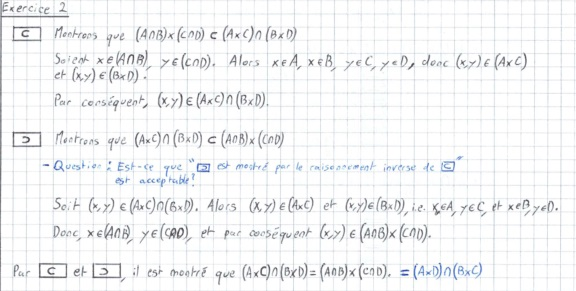
\includegraphics{ex02.jpg}
	
	\newpage
	
	\noindent
	\textbf{Exercice 3.}\\
	Considérons le système d'équations linéaires suivant pour les
	inconnues $x, y$ et $z$ :
	\[\left\{\begin{matrix}[rrrcl]
		mx & +y & +z &=& 1\\
		x & +my & +z &=& m\\
		x & +y & +mz &=& m^2\\
	\end{matrix}\right.\]
	\begin{enumerate}[label=(\roman*)]
		\item Résoudre ce système linéaire pour le cas particulier $m = 0$
		%
		\item Résoudre ce système linéaire pour le cas particulier $m = -1$
		%
		\item Plus généralement, pour quelles valeur de $m \in \mathbb{R}$
		ce système possède-t-il une solution ?\\
		Dans le cas où une solution existe, est-elle unique ?
	\end{enumerate}
	
	\colorbox{solution}
	{\begin{minipage}{0.9\textwidth}
		
	\end{minipage}}
	
	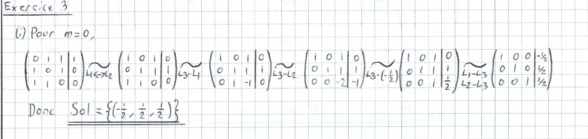
\includegraphics{ex03-p1.jpg}
	
	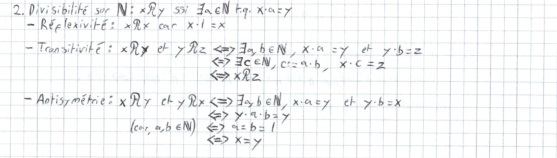
\includegraphics{ex03-p2.jpg}
	
	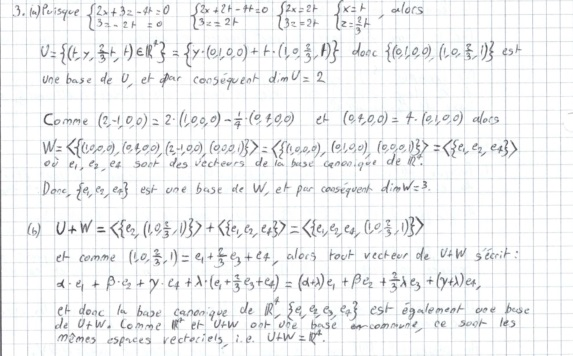
\includegraphics{ex03-p3.jpg}
	
	\newpage
	
	\noindent
	\textbf{Exercice 4.}\\
	Considérons les vecteurs suivants de $\mathbb{R}^3$ :
	\[
		u_1 = (1, 2, 3), \quad u_1 = (4, 5, 6), \quad u_1 = (1, -1, 0)
	\]
	\begin{enumerate}[label=(\roman*)]
		\item À l'aide de la méthode du pivot. montrer que
		$\{u_1, u_2, u_3\}$ est une base de $\mathbb{R}^3$
		%
		\item À l'aide de la méthode du pivot, écrire $(1, 3, -6)$
		dans la base $\{u_1, u_2, u_3\}$
		%
		\item On note $F$ le sous-espace vectoriel de $\mathbb{R}^3$
		engendré par $u_1$ et $u_2$.\\
		Écrire $F$ sous la forme
		\[
		F = \{(x_1 x_2 x_3) \in \mathbb{R}^3 \mid ax_1 + bx_2 + cx_3 = d\}
		\]
		où $a, b, c, d$ sont des réels à préciser.\\
		\textit{Indications : Un sous-espace de $\mathbb{R}^3$ généré par
			deux vecteurs non-colinéaires forme un plan. Un plan peut être
			décrit par son équation cartésienne $ax + by + cz = d$. Ici,
			par définition d’un sous-espace	vectoriel, $(0, 0, 0) \in F.$
			Par définition de $F$, on a également $u_1, u_2 \in F$.\\
			Avec ces informations, peut-on déterminer les coefficients
			$a, b, c$ et $d$ ?}
	\end{enumerate}
	
	\colorbox{solution}
	{\begin{minipage}{0.9\textwidth}
		\begin{enumerate}[label=(\roman*)]
			\item Observons la matrice $A = (u_1\ u_2\ u_3)$ :
			\[\footnotesize
			\begin{pmatrix}[rrr]
				1 & 4 & 1\\
				2 & 5 & -1\\
				3 & 6 & 0
			\end{pmatrix}
			\underset{\substack{L_2 - 2L_1 \\ L_3 - 3L_1}}{\sim}
			\begin{pmatrix}[rrr]
				1 & 4 & 1\\
				0 & -3 & -3\\
				0 & -6 & -3
			\end{pmatrix}
			\underset{\substack{L_3 - 2L_2}}{\sim}
			\begin{pmatrix}[rrr]
				1 & 4 & 1\\
				0 & -3 & -3\\
				0 & 0 & 3
			\end{pmatrix}\]
			On constate que la forme échelonnée de $A$ met en évidence
			3 pivots. Ainsi, le système linéaire
			$a_1u_1 + a_2u_2 +a_3u_3 = b$ admet une unique solution pour
			n'importe quel vecteur $b \in \mathbb{R}^3$.\\
			
			On en conclut que les vecteurs colonne de
			$A\ (i.e. \{u_1, u_2, u_3\})$ forment une base de
			$\mathbb{R}^3$.
			%
			\item \[\footnotesize
				\begin{pmatrix}[rrr|r]
				1 & 4 & 1 & 1\\[0.3em]
				2 & 5 & -1 & 3\\[0.3em]
				3 & 6 & 0 & -6
			\end{pmatrix}
			\underset{\substack{L_2 - 2L_1 \\ L_3 - 3L_1}}{\sim}
			\begin{pmatrix}[rrr|r]
				1 & 4 & 1 & 1\\[0.3em]
				0 & -3 & -3 & 1\\[0.3em]
				0 & -6 & -3 & -9
			\end{pmatrix}
			\underset{\substack{L_3 - 2L_2}}{\sim}
			\begin{pmatrix}[rrr|r]
				1 & 4 & 1 & 1\\[0.3em]
				0 & -3 & -3 & 1\\[0.3em]
				0 & 0 & 3 & -11
			\end{pmatrix}
			\underset{\substack{L_2 \cdot (-\frac{1}{3})\\
					L_3 \cdot \frac{1}{3}}}{\sim}
			\]\[\footnotesize
			\begin{pmatrix}[rrr|l]
				1 & 4 & 1 & 1\\[0.3em]
				0 & 1 & 1 & -\frac{1}{3}\\[0.3em]
				0 & 0 & 1 & -\frac{11}{3}
			\end{pmatrix}
			\underset{\substack{L_1 - L_3 \\ L_2 - L_3}}{\sim}
			\begin{pmatrix}[rrr|r]
				1 & 4 & 0 & \frac{14}{3}\\[0.3em]
				0 & 1 & 0 & \frac{10}{3}\\[0.3em]
				0 & 0 & 1 & -\frac{11}{3}
			\end{pmatrix}
			\underset{\substack{L_1 - 4L_2}}{\sim}
			\begin{pmatrix}[rrr|r]
				1 & 0 & 0 & -\frac{26}{3}\\[0.3em]
				0 & 1 & 0 & \frac{10}{3}\\[0.3em]
				0 & 0 & 1 & -\frac{11}{3}
			\end{pmatrix}
			\]
						
			Les coordonnées de $(1, 3, -6)$ dans la base $\{u_1, u_2, u_3\}$
			sont donc $(-\frac{26}{3}, \frac{10}{3}, -\frac{11}{3})$.
		\end{enumerate}
	\end{minipage}}
	
	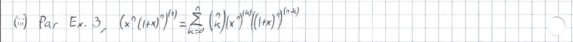
\includegraphics{ex04-p3.jpg}
	
	\newpage
	
	\noindent
	\textbf{Exercice 5.}\\
	Considérons $\mathbb{R}_2[x]$ l'espace des polynômes de degré
	inférieur ou égal à 2.
	\begin{enumerate}[label=(\roman*)]
		\item À l'aide de la méthode du pivot. montrer que
		$\mathcal{B} = \{1 + 2x + 3x^2, 4 + 5x + 6x^2, 1 -x\}$
		est une base de $\mathbb{R}_2[x]$
		%
		\item À l'aide de la méthode du pivot, écrire $1 + 3x -6x^2$
		comme combinaison linéaire des éléments de $\mathcal{B}$
		%
		\item On note $F$ le sous-espace vectoriel de $\mathbb{R}_2[x]$
		engendré par $1 + 2x + 3x^2$ et $4 + 5x + 6x^2$.\\
		Écrire $F$ sous la forme
		\[
		F = \{\alpha_0 + \alpha_1x + \alpha_2x^2 \in \mathbb{R}_2[x]
			\mid a\alpha_0 + b\alpha_1 + c\alpha_2 = d\}
		\]
		où $a, b, c, d$ sont des réels à préciser.
	\end{enumerate}
	
	\colorbox{solution}
	{\begin{minipage}{0.9\textwidth}
		\textit{\color{blue} Est-ce qu'il y a un point que je ne
		remarque pas, où c'est exactement le même exercice que
		Exercice 4 ?}\\
		
		\begin{enumerate}[label=(\roman*)]
			\item Même démonstration que 4.(i)
			%
			\item $1 + 3x -6x^2 = -\frac{26}{3} \cdot (1 + 2x + 3x^2) +
				\frac{10}{3} \cdot (4 + 5x + 6x^2) -
				\frac{11}{3} \cdot (1 - x)$
			%
			\item $F = \{\alpha_0 + \alpha_1x + \alpha_2x^2 \in \mathbb{R}_2[x]
			\mid \alpha_0 - 2\alpha_1 + \alpha_2 = 0\}$
		\end{enumerate}
	\end{minipage}}
	
%	
%	\colorbox{solution}
%	{
%		\begin{minipage}{0.9\textwidth}
%			s
%		\end{minipage}
%	}
%	
%	\colorbox{solution}
%	{
%		\begin{minipage}{0.9\textwidth}
%			\begin{enumerate}[label=(\alph*)]
%				\item a
%			\end{enumerate}
%		\end{minipage}
%	}
	
\end{document}
